\documentclass{standalone}
\usepackage{tikz}
\usetikzlibrary{patterns, positioning}
\usepackage[sfdefault]{ClearSans} %% option 'sfdefault' activates Clear Sans as the default text font
\usepackage[T1]{fontenc}

\begin{document}
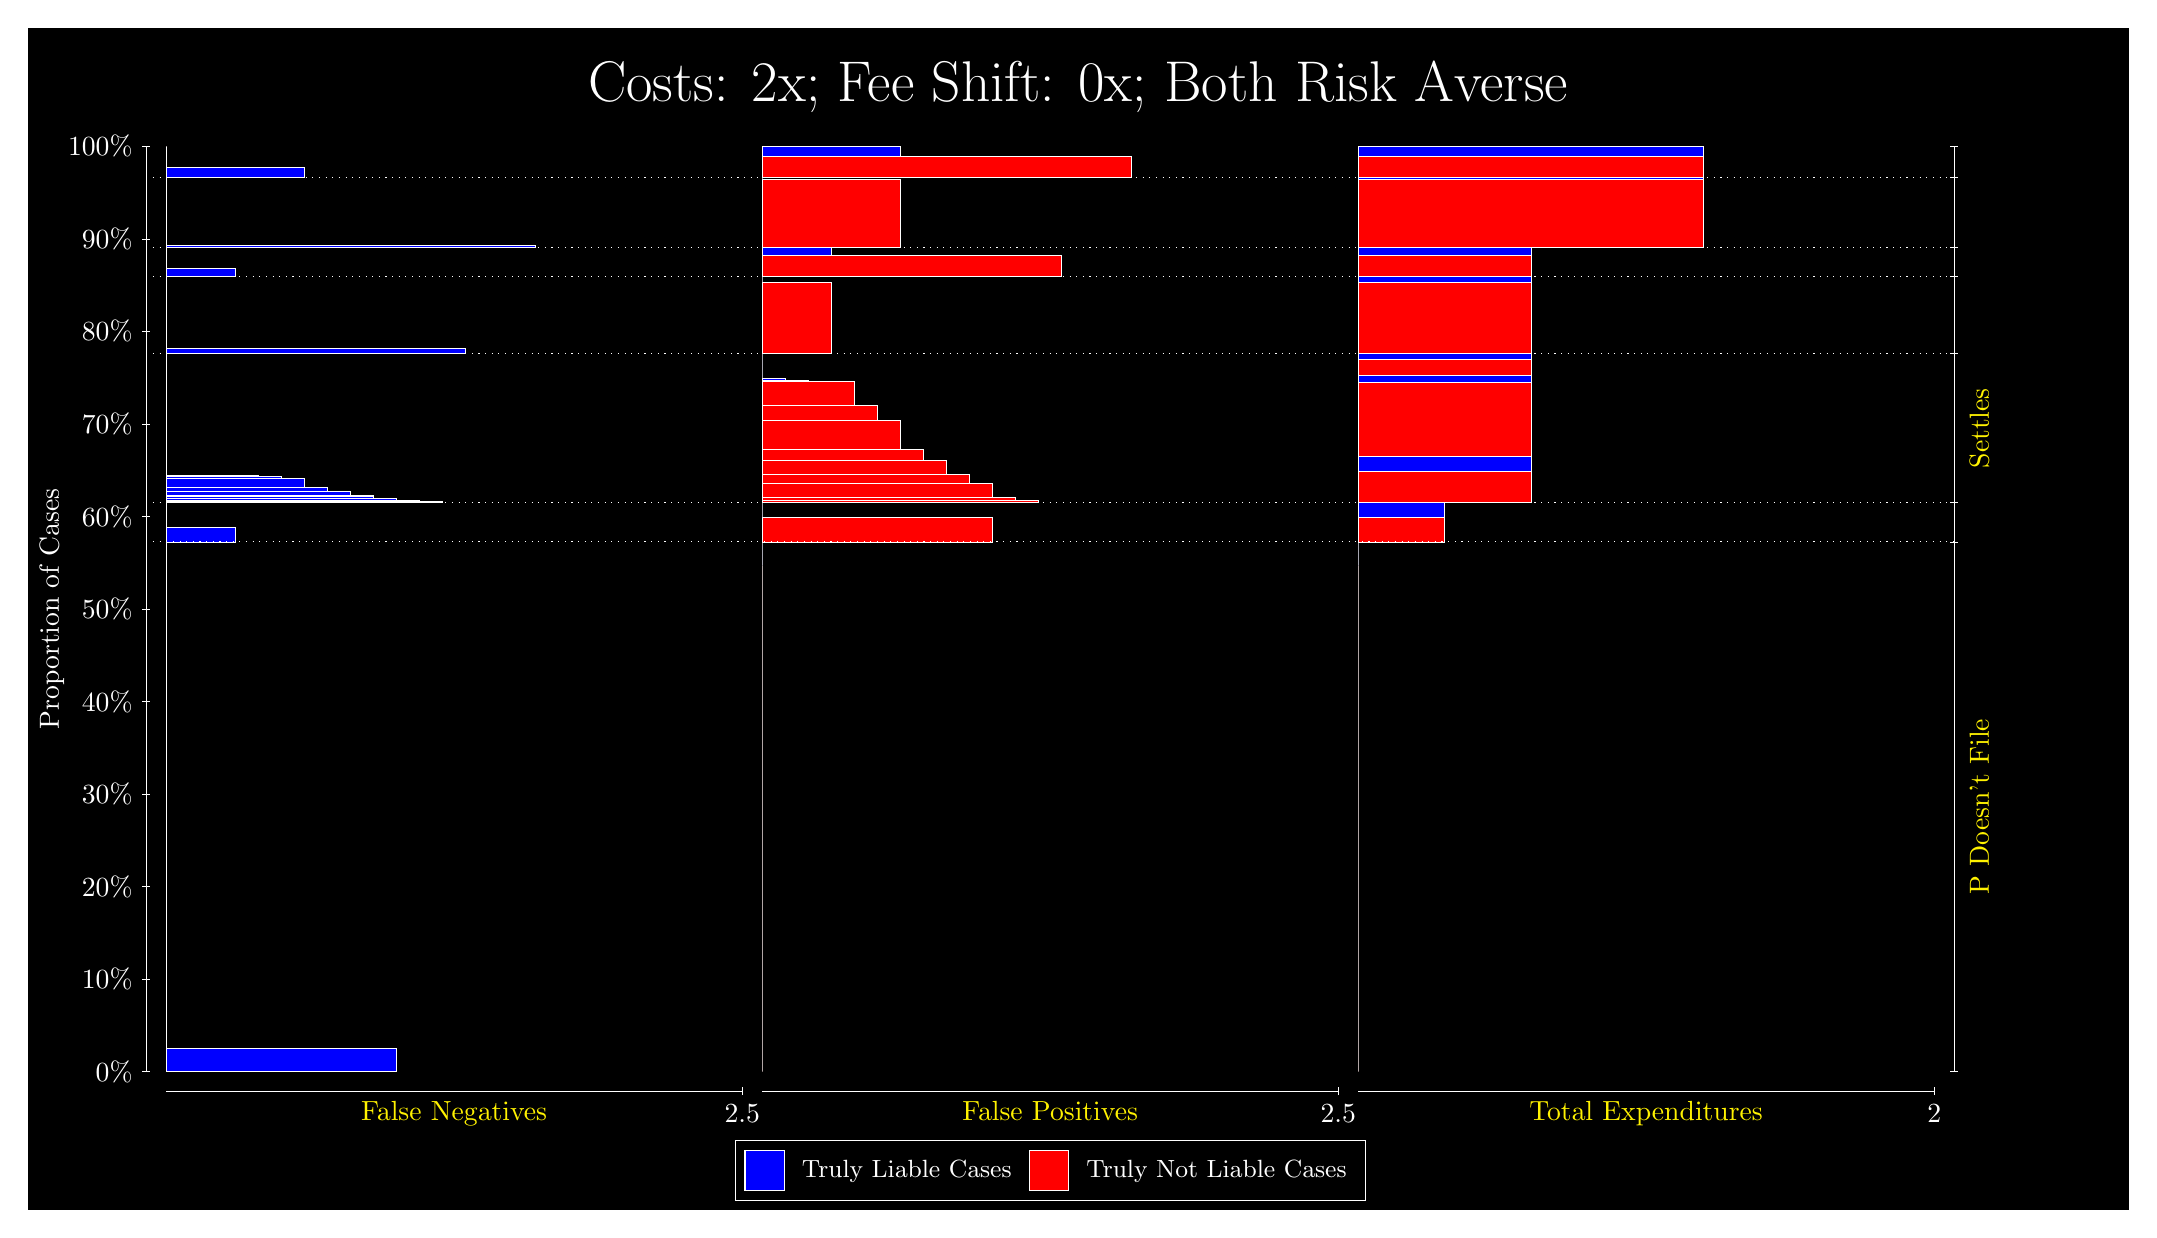
\begin{tikzpicture}
\draw[fill=black] (0,0) rectangle (26.667,15);
\draw[text=white] (0,13.5) rectangle (26.667,15) node[midway] {\huge Costs: 2x; Fee Shift: 0x; Both Risk Averse};
\draw[white, very thin] (1.5,1.75) -- (1.5,13.5);
\node[rotate=90, text=white, anchor=center] at (0.3, 7.625) {Proportion of Cases};
\draw[white, very thin] (1.45,1.75) -- (1.55,1.75);
\node[text=white, anchor=east] at (1.45, 1.75) {0\%};
\draw[white, very thin] (1.45,2.925) -- (1.55,2.925);
\node[text=white, anchor=east] at (1.45, 2.925) {10\%};
\draw[white, very thin] (1.45,4.1) -- (1.55,4.1);
\node[text=white, anchor=east] at (1.45, 4.1) {20\%};
\draw[white, very thin] (1.45,5.275) -- (1.55,5.275);
\node[text=white, anchor=east] at (1.45, 5.275) {30\%};
\draw[white, very thin] (1.45,6.45) -- (1.55,6.45);
\node[text=white, anchor=east] at (1.45, 6.45) {40\%};
\draw[white, very thin] (1.45,7.625) -- (1.55,7.625);
\node[text=white, anchor=east] at (1.45, 7.625) {50\%};
\draw[white, very thin] (1.45,8.8) -- (1.55,8.8);
\node[text=white, anchor=east] at (1.45, 8.8) {60\%};
\draw[white, very thin] (1.45,9.975) -- (1.55,9.975);
\node[text=white, anchor=east] at (1.45, 9.975) {70\%};
\draw[white, very thin] (1.45,11.15) -- (1.55,11.15);
\node[text=white, anchor=east] at (1.45, 11.15) {80\%};
\draw[white, very thin] (1.45,12.325) -- (1.55,12.325);
\node[text=white, anchor=east] at (1.45, 12.325) {90\%};
\draw[white, very thin] (1.45,13.5) -- (1.55,13.5);
\node[text=white, anchor=east] at (1.45, 13.5) {100\%};

\draw[white, very thin] (24.457,1.75) -- (24.457,13.5);
\draw[white, very thin] (24.407,1.75) -- (24.507,1.75);
\node[anchor=west] at (24.407, 1.75) {};
\draw[white, very thin] (24.407,8.4773) -- (24.507,8.4773);
\node[anchor=west] at (24.407, 8.4773) {};
\draw[white, very thin] (24.407,8.9738) -- (24.507,8.9738);
\node[anchor=west] at (24.407, 8.9738) {};
\draw[white, very thin] (24.407,10.868) -- (24.507,10.868);
\node[anchor=west] at (24.407, 10.868) {};
\draw[white, very thin] (24.407,11.846) -- (24.507,11.846);
\node[anchor=west] at (24.407, 11.846) {};
\draw[white, very thin] (24.407,12.218) -- (24.507,12.218);
\node[anchor=west] at (24.407, 12.218) {};
\draw[white, very thin] (24.407,13.108) -- (24.507,13.108);
\node[anchor=west] at (24.407, 13.108) {};
\draw[white, very thin] (24.407,13.5) -- (24.507,13.5);
\node[anchor=west] at (24.407, 13.5) {};

\draw[white, very thin, fill=blue] (1.75,1.75) rectangle (4.6775,2.0501);
\draw[white, very thin, fill=red] (1.75,2.0501) rectangle (1.75,8.4773);
\draw[white, very thin, fill=blue] (1.75,8.4773) rectangle (2.6283,8.6676);
\draw[white, very thin, fill=red] (1.75,8.6676) rectangle (1.75,8.9738);
\draw[white, very thin, fill=blue] (1.75,8.9738) rectangle (5.2631,8.99);
\draw[white, very thin, fill=blue] (1.75,8.99) rectangle (4.9703,9.0047);
\draw[white, very thin, fill=blue] (1.75,9.0047) rectangle (4.6775,9.0349);
\draw[white, very thin, fill=blue] (1.75,9.0349) rectangle (4.3848,9.0588);
\draw[white, very thin, fill=blue] (1.75,9.0588) rectangle (4.3848,9.0724);
\draw[white, very thin, fill=blue] (1.75,9.0724) rectangle (4.092,9.1239);
\draw[white, very thin, fill=blue] (1.75,9.1239) rectangle (3.7993,9.1689);
\draw[white, very thin, fill=blue] (1.75,9.1689) rectangle (3.5065,9.2854);
\draw[white, very thin, fill=blue] (1.75,9.2854) rectangle (3.2138,9.3136);
\draw[white, very thin, fill=blue] (1.75,9.3136) rectangle (2.921,9.3265);
\draw[white, very thin, fill=red] (1.75,9.3265) rectangle (1.75,10.868);
\draw[white, very thin, fill=blue] (1.75,10.868) rectangle (5.5558,10.939);
\draw[white, very thin, fill=red] (1.75,10.939) rectangle (1.75,11.846);
\draw[white, very thin, fill=blue] (1.75,11.846) rectangle (2.6283,11.948);
\draw[white, very thin, fill=red] (1.75,11.948) rectangle (1.75,12.218);
\draw[white, very thin, fill=blue] (1.75,12.218) rectangle (6.4341,12.247);
\draw[white, very thin, fill=red] (1.75,12.247) rectangle (1.75,13.108);
\draw[white, very thin, fill=blue] (1.75,13.108) rectangle (3.5065,13.238);
\draw[white, very thin, fill=red] (1.75,13.238) rectangle (1.75,13.5);
\draw[white, very thin, fill=red] (9.3189,1.75) rectangle (9.3189,8.1772);
\draw[white, very thin, fill=blue] (9.3189,8.1772) rectangle (9.3189,8.4773);
\draw[white, very thin, fill=red] (9.3189,8.4773) rectangle (12.246,8.7834);
\draw[white, very thin, fill=blue] (9.3189,8.7834) rectangle (9.3189,8.9738);
\draw[white, very thin, fill=red] (9.3189,8.9738) rectangle (12.832,8.9996);
\draw[white, very thin, fill=red] (9.3189,8.9996) rectangle (12.539,9.0465);
\draw[white, very thin, fill=red] (9.3189,9.0465) rectangle (12.246,9.2254);
\draw[white, very thin, fill=red] (9.3189,9.2254) rectangle (11.954,9.3376);
\draw[white, very thin, fill=red] (9.3189,9.3376) rectangle (11.661,9.5096);
\draw[white, very thin, fill=red] (9.3189,9.5096) rectangle (11.368,9.65);
\draw[white, very thin, fill=red] (9.3189,9.65) rectangle (11.075,10.017);
\draw[white, very thin, fill=red] (9.3189,10.017) rectangle (10.783,10.209);
\draw[white, very thin, fill=red] (9.3189,10.209) rectangle (10.49,10.515);
\draw[white, very thin, fill=blue] (9.3189,10.515) rectangle (9.9044,10.528);
\draw[white, very thin, fill=blue] (9.3189,10.528) rectangle (9.6116,10.556);
\draw[white, very thin, fill=blue] (9.3189,10.556) rectangle (9.3189,10.868);
\draw[white, very thin, fill=red] (9.3189,10.868) rectangle (10.197,11.776);
\draw[white, very thin, fill=blue] (9.3189,11.776) rectangle (9.3189,11.846);
\draw[white, very thin, fill=red] (9.3189,11.846) rectangle (13.125,12.116);
\draw[white, very thin, fill=blue] (9.3189,12.116) rectangle (10.197,12.218);
\draw[white, very thin, fill=red] (9.3189,12.218) rectangle (11.075,13.079);
\draw[white, very thin, fill=blue] (9.3189,13.079) rectangle (9.3189,13.108);
\draw[white, very thin, fill=red] (9.3189,13.108) rectangle (14.003,13.37);
\draw[white, very thin, fill=blue] (9.3189,13.37) rectangle (11.075,13.5);
\draw[white, very thin, fill=red] (16.888,1.75) rectangle (16.888,8.1772);
\draw[white, very thin, fill=blue] (16.888,8.1772) rectangle (16.888,8.4773);
\draw[white, very thin, fill=red] (16.888,8.4773) rectangle (17.986,8.7834);
\draw[white, very thin, fill=blue] (16.888,8.7834) rectangle (17.986,8.9738);
\draw[white, very thin, fill=red] (16.888,8.9738) rectangle (19.083,9.3716);
\draw[white, very thin, fill=blue] (16.888,9.3716) rectangle (19.083,9.5677);
\draw[white, very thin, fill=red] (16.888,9.5677) rectangle (19.083,10.504);
\draw[white, very thin, fill=blue] (16.888,10.504) rectangle (19.083,10.589);
\draw[white, very thin, fill=red] (16.888,10.589) rectangle (19.083,10.796);
\draw[white, very thin, fill=blue] (16.888,10.796) rectangle (19.083,10.868);
\draw[white, very thin, fill=red] (16.888,10.868) rectangle (19.083,11.776);
\draw[white, very thin, fill=blue] (16.888,11.776) rectangle (19.083,11.846);
\draw[white, very thin, fill=red] (16.888,11.846) rectangle (19.083,12.116);
\draw[white, very thin, fill=blue] (16.888,12.116) rectangle (19.083,12.218);
\draw[white, very thin, fill=red] (16.888,12.218) rectangle (21.279,13.079);
\draw[white, very thin, fill=blue] (16.888,13.079) rectangle (21.279,13.108);
\draw[white, very thin, fill=red] (16.888,13.108) rectangle (21.279,13.37);
\draw[white, very thin, fill=blue] (16.888,13.37) rectangle (21.279,13.5);
\draw[white, dotted] (1.5,8.4773) -- (24.457,8.4773);
\draw[white, dotted] (1.5,8.9738) -- (24.457,8.9738);
\draw[white, dotted] (1.5,10.868) -- (24.457,10.868);
\draw[white, dotted] (1.5,11.846) -- (24.457,11.846);
\draw[white, dotted] (1.5,12.218) -- (24.457,12.218);
\draw[white, dotted] (1.5,13.108) -- (24.457,13.108);
\draw[white, very thin] (1.75,1.5) -- (9.0689,1.5);
\node[text=yellow, anchor=north] at (5.4094, 1.5) {False Negatives};
\draw[white, very thin] (9.0689,1.45) -- (9.0689,1.55);
\node[text=white, anchor=north] at (9.0689, 1.45) {2.5};

\draw[white, very thin] (9.3189,1.5) -- (16.638,1.5);
\node[text=yellow, anchor=north] at (12.978, 1.5) {False Positives};
\draw[white, very thin] (16.638,1.45) -- (16.638,1.55);
\node[text=white, anchor=north] at (16.638, 1.45) {2.5};

\draw[white, very thin] (16.888,1.5) -- (24.207,1.5);
\node[text=yellow, anchor=north] at (20.547, 1.5) {Total Expenditures};
\draw[white, very thin] (24.207,1.45) -- (24.207,1.55);
\node[text=white, anchor=north] at (24.207, 1.45) {2};

\node[text=yellow, centered, rotate=90] at (24.777, 5.1136) {P Doesn't File};

\node[text=yellow, centered, rotate=90] at (24.777, 9.9208) {Settles};





\draw (12.978300999999998,1.5) node[draw=none] (baseCoordinate) {};
\begin{scope}[align=center]
        \matrix[scale=0.5, draw=white, below=0.5cm of baseCoordinate, nodes={draw}, column sep=0.1cm]{
            \node[rectangle, draw, minimum width=0.5cm, minimum height=0.5cm, fill=blue] {}; &
            \node[draw=none, font=\small, text=white] (B) {Truly Liable Cases}; &
            \node[rectangle, draw, minimum width=0.5cm, minimum height=0.5cm, fill=red] {}; &
            \node[draw=none, font=\small, text=white] (B) {Truly Not Liable Cases}; \\
            };
\end{scope}

\end{tikzpicture}
\end{document}